%% ---------------------------
% Zusätzliche Pakete und Definitionen
%% ---------------------------

\usepackage[utf8]{inputenc}
\usepackage[ngerman]{babel} % Sprachanpassungen und Trennmuster
\usepackage[T1]{fontenc}    % T1 Schrift Encoding
\usepackage{textcomp}       % zusätzliche Symbole (Text Companion)
\usepackage{mathptmx}              %% --- Times mit Matheschriften
% \usepackage{mathpazo}            %% --- Palatino
\usepackage[scaled=.90]{helvet}    %% --- Helvetica

\usepackage{booktabs}
\usepackage{multimedia}
\usepackage{listings}
\usepackage{enumerate}
%% ---------------------------
% Beamer Theme
%% ---------------------------
\usetheme{Esslingen}

%\usecolortheme{default}  %      kein Farb-Hintergrund in Blöcken
%\usecolortheme{lily}     %      kein Farb-Hintergrund in Blöcken
 \usecolortheme{rose}     %  dezenter Farb-Hintergrund in Blöcken
%\usecolortheme{orchid}   % kräftiger Farb-Hintergrund in Blöcken

\setbeamercovered{transparent=30}

\vspace*{1ex}

%% ---------------------------
%% Definitionen für die Titelseite
%% ---------------------------
%% Die optionalen Argumente werden für die Fußzeile benutzt

\title{Distributed Real-Time Systems}

%\subtitle[Beispiel-Dokument]{Ein einfaches Beispiel-Dokument}

\author{Prof. Dr. Joerg Friedrich\inst{1}
\and
 %Zweiter Autor\inst{1} \and
 %Dritter Autor\inst{2}
 }

\titlegraphic{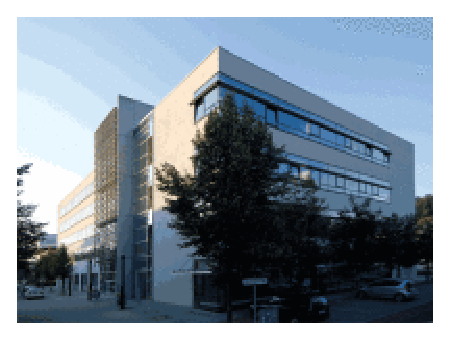
\includegraphics[scale=0.5]{figures/HEGoeppingen}}


\institute[Hochschule Esslingen]{%
\inst{1}Hochschule Esslingen, Faculty of Computer Science
 % \and
 %\inst{2}Andere Einrichtung
 }

\date[\copyright{} 2011]{\today}

